% !TEX root = paper.tex

\section {Results}
\label{sec:results}

\subsection{Ridge yield}
\label{sec:resultunbiased}
\begin{figure}[b!]
	\centering
	\subfigure{ 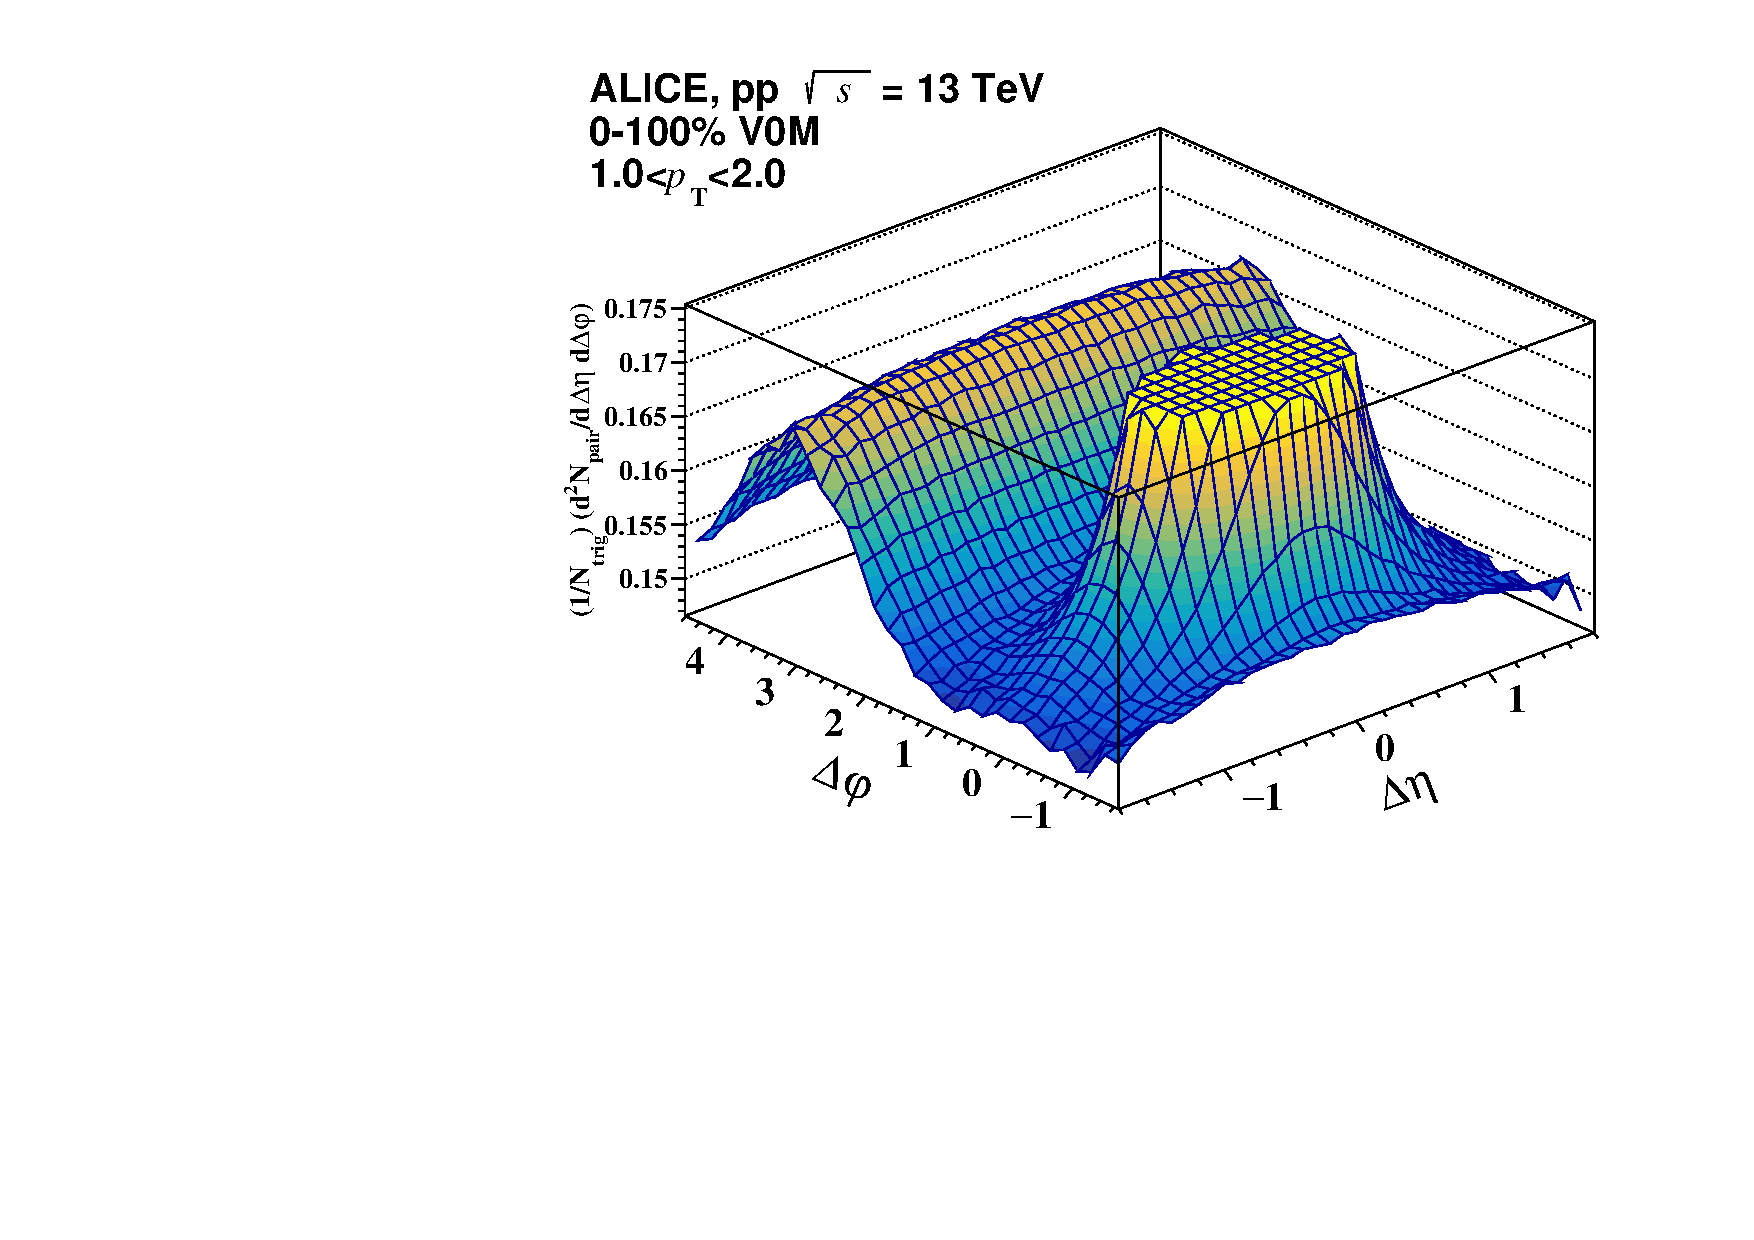
\includegraphics[width=0.47 \textwidth]{./figures/corrmb.pdf} }
	\subfigure{ 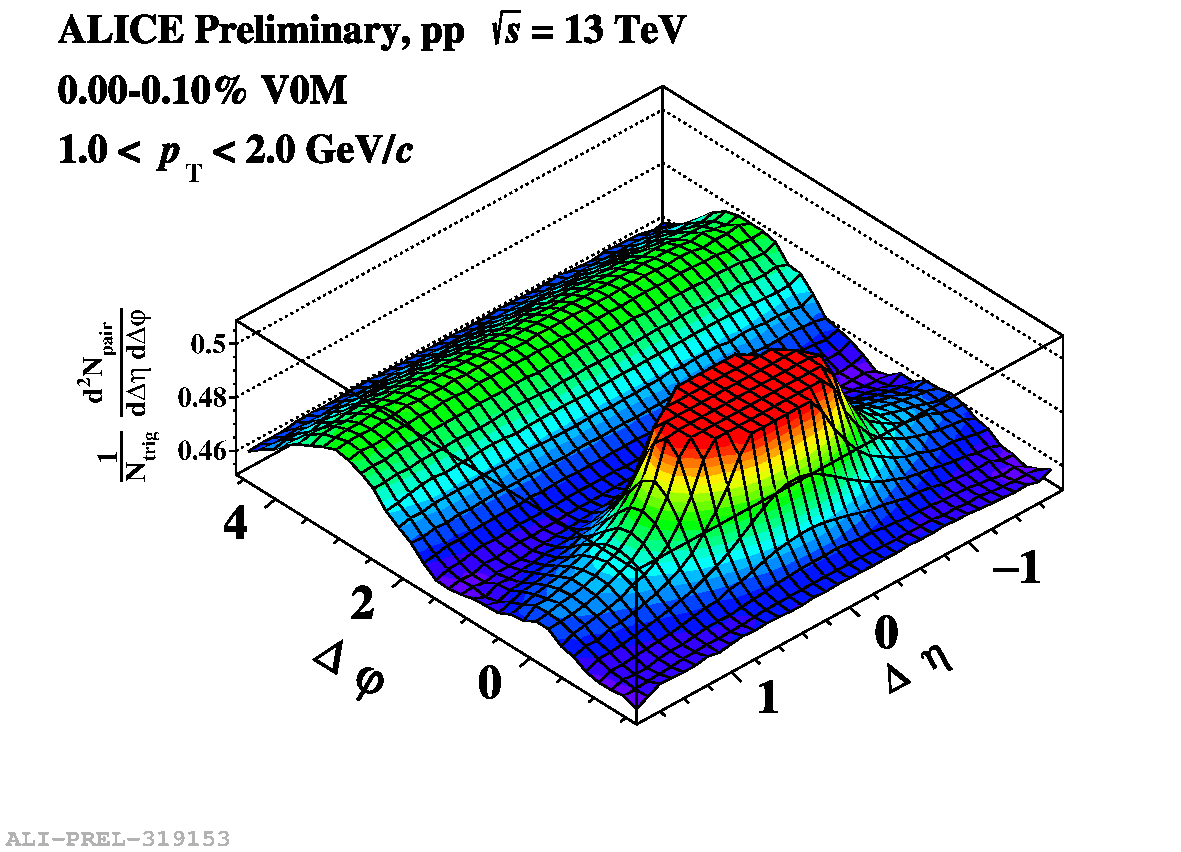
\includegraphics[width=0.47 \textwidth]{./figures/corr1.pdf} }
	\caption{ Two-particle correlation functions as functions of $\Delta\eta$ and $\Delta\varphi$ in minimum-bias events (0--100\%, left) and high-multiplicity (0--0.1\%, right). Note that the near-side jet peaks exceed the chosen range of the $z$-axis. The intervals of $\pttrig$ and $\ptassoc$ are 1~$<\it{p}_{\rm{T}}<$~2~GeV/$c$ in both cases.}
	\label{fig:PlotCorrMBHMT}
\end{figure}

Figure~\ref{fig:PlotCorrMBHMT} shows the per-trigger yield obtained from Eq.~(1) for 1~$<\pttrig~\mathrm (\ptassoc)<$~2 GeV/$c$ in pp collisions at $\sqrt{\it{s}} = $\unit{13} {\rm{}TeV} for minimum bias events (left) and high-multiplicity (right). It is worth noting that the $z$-axes for the yield of the correlations is properly scaled in order to zoom in the ridge yield, as a result, the jet peaks are sheared off in both figures. The ridge structure is clearly observed in the high-multiplicity class while it is less significant in the minimum bias events. The away-side yield is populated mostly by back-to-back jet correlations.

\begin{figure}[h!]
	\centering
	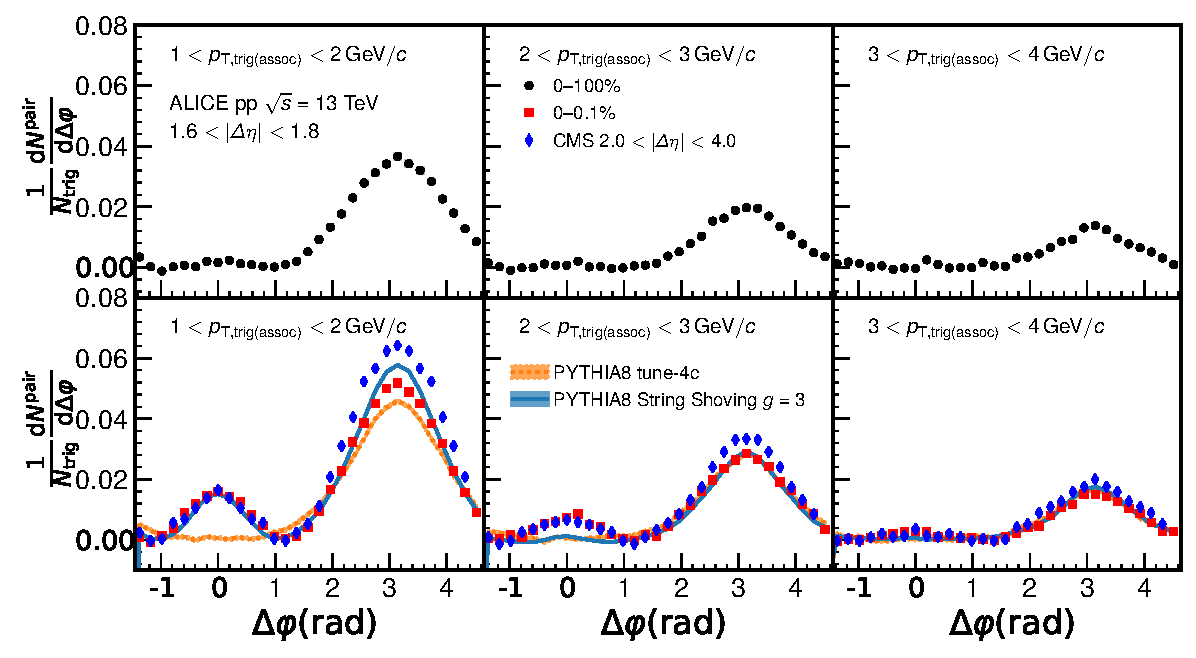
\includegraphics[width=0.9\linewidth]{./figures/Fig2_PlotDeltaPhi.pdf}
	\caption{One-dimensional $\Delta\varphi$ distribution in the large $\Delta\eta$ projection for three transverse momentum intervals in minimum bias (upper panels) and high-multiplicity (lower panels) events after ZYAM subtraction. Transverse momentum intervals of the trigger particles and associated particles are 1~$<\pt<$~2 (left), 2~$<\pt<$~3 (middle) and, 3~$<\pt<$~4 GeV/$c$ (right), respectively. The presented model predictions were calculated using $\pythiashoving$, $\pythiam$, and $\epos$.}
	\label{fig:PlotDeltaPhi}
\end{figure}
 
Figure~\ref{fig:PlotDeltaPhi} shows $\Delta\varphi$ projections of the two-particle correlation functions obtained in the range 1.6~$<|\Delta \eta |<$~1.8 for several track $\pt$ intervals after the ZYAM subtraction (see Eq.~(2)). The results are shown for various $\it{p}_{\rm{T}}$ intervals in the minimum bias class (upper) and the high-multiplicity class (lower) down to 1~GeV/$c$ where the non-flow contamination is negligible. The near-side ($\Delta\varphi\sim 0$) ridge in the high-multiplicity class is clearly observed for $\pt<$~3~GeV/$c$ while there is no definitive signal in the minimum bias class. Within the range of analyzed particle $\pt$, the yield in the near-side ridge decreases with increasing $\pt$ in the high-multiplicity class.

The measurements in the high-multiplicity class are compared with the results published by the CMS Collaboration~\cite{Khachatryan:2015lva}. In case of the CMS measurement, the charged particle multiplicity was obtained by counting the number of particles satisfying $\pt>0.4$~GeV/$c$ in $|\eta|<$~2.4. In our analysis, event multiplicity is determined from the forward V0 detectors. The difference in multiplicity selection between ALICE (forward) and CMS (midrapidity) is studied using PYTHIA~8 simulations and it is found that the calculated multiplicity using the CMS procedure is about 20\% larger than the one from ALICE when compared in the acceptance region of the measurements reported in this article, $|\eta|<$~0.9. Near-side ridges in all transverse momentum ranges are comparable. The larger away-side yields observed in \cite{Khachatryan:2015lva} can be attributed to the difference in $\eta$ acceptance for the multiplicity selection, which overlaps somewhat with the $\eta$ region in Fig.~\ref{fig:PlotDeltaPhi} for the CMS results.

In Fig.~\ref{fig:PlotDeltaPhi}, the ALICE measurements are also compared with model predictions where a comparable high-multiplicity selection and $\Delta\eta$ projection range are applied. The selection of high-multiplicity events in the models is done by requiring a minimal number of charged particles emitted within the V0M detector acceptance. In case of $\pythiam$, the 0--0.1\% centrality threshold is 105 charged particles. The threshold for $\epos$ and $\pythiashoving$ are 110 and 108, respectively. The magnitude of string shoving ($g$) is set to 3.0 in this study. The statistical uncertainties due to the limited number of events for the model calculations are shown as bands in each figure. The $\pythiashoving$ provides good estimates of the near-side ridge yield and slightly overestimates the away-side yield for the interval 1~$<\it{p}_{\rm{T}}<$~2~GeV/$c$. However, the $\pythiashoving$ model underestimates the near-side ridge yield for $\it{p}_{\rm{T}}>$~2~GeV/$c$. The $\pythiam$ model does not show any near-side ridge as expected. It slightly underestimates the away-side peak for 1~$<\it{p}_{\rm{T}}<$~2~GeV/$c$ and provides good estimates for $\it{p}_{\rm{T}}>$~2~GeV/$c$. On the other hand, $\epos$ describes the shape of the ridge yield quantitatively better in the 2~$<\pttrigassoc<$~4~GeV/$c$ range, while overestimating the near-side ridge yield for $\pttrigassoc<$~2~GeV/$c$ range. 


\begin{figure}[h!]
	\centering
	\subfigure{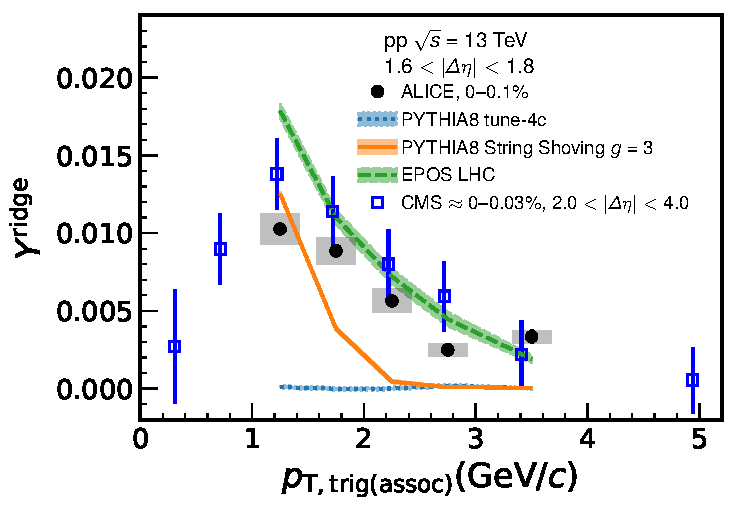
\includegraphics[width=0.89\textwidth]{./figures/Fig3_PlotRidgeYield.pdf}}
	\caption{ Fully corrected near-side ridge yield as a function transverse momentum. The open blue boxes denote the measurement by ALICE. The statistical and systematic uncertainties are shows as vertical bars and boxes, respectively. The CMS measurement~\cite{Khachatryan:2015lva} is represented by filled circles and extends down to lower $\pt$ due to the larger $\Delta\eta$ acceptance. The three lines show model predictions from $\pythiam$ (blue dotted line), $\pythiashoving$ (orange line) and, $\epos$ (green dashed line).}
	\label{fig:PlotYSpect}
\end{figure}

Figure~\ref{fig:PlotYSpect} shows the near-side ridge yield measured in high-multiplicity events as a function of $\pttrigassoc$. The measurement is compared with the result from CMS~\cite{Khachatryan:2015lva}.
%The ridge yields as a function of the transverse momentum are shown in Fig.~\ref{fig:PlotYSpect} in the high-multiplicity class and compared to \cite{Khachatryan:2015lva}.
Considering the differences in acceptance and the chosen multiplicity estimator of both measurements, perfect agreement between the two sets of results is not expected. The measurement is also compared with model calculations. As expected, the PYTHIA~8 model with Tune 4C does not produce a near-side ridge because it is not designed to account for this effect. The $\pythiashoving$ model describes the yield qualitatively, however the predicted yield decreases more rapidly than the measured one for increasing $\pttrigassoc$. The $\epos$ model, unlike the $\pythiashoving$ model, describes well the $\pt$ dependence of the ridge yield for the range $\it{p}_{\rm{T}}>$~2~GeV/$c$ , while predicting larger yields for $\it{p}_{\rm{T}}<$~2 GeV/$c$.

\subsection{Event-scale dependence of the ridge yield}
\begin{figure}[h!]
	\centering
	\subfigure{ 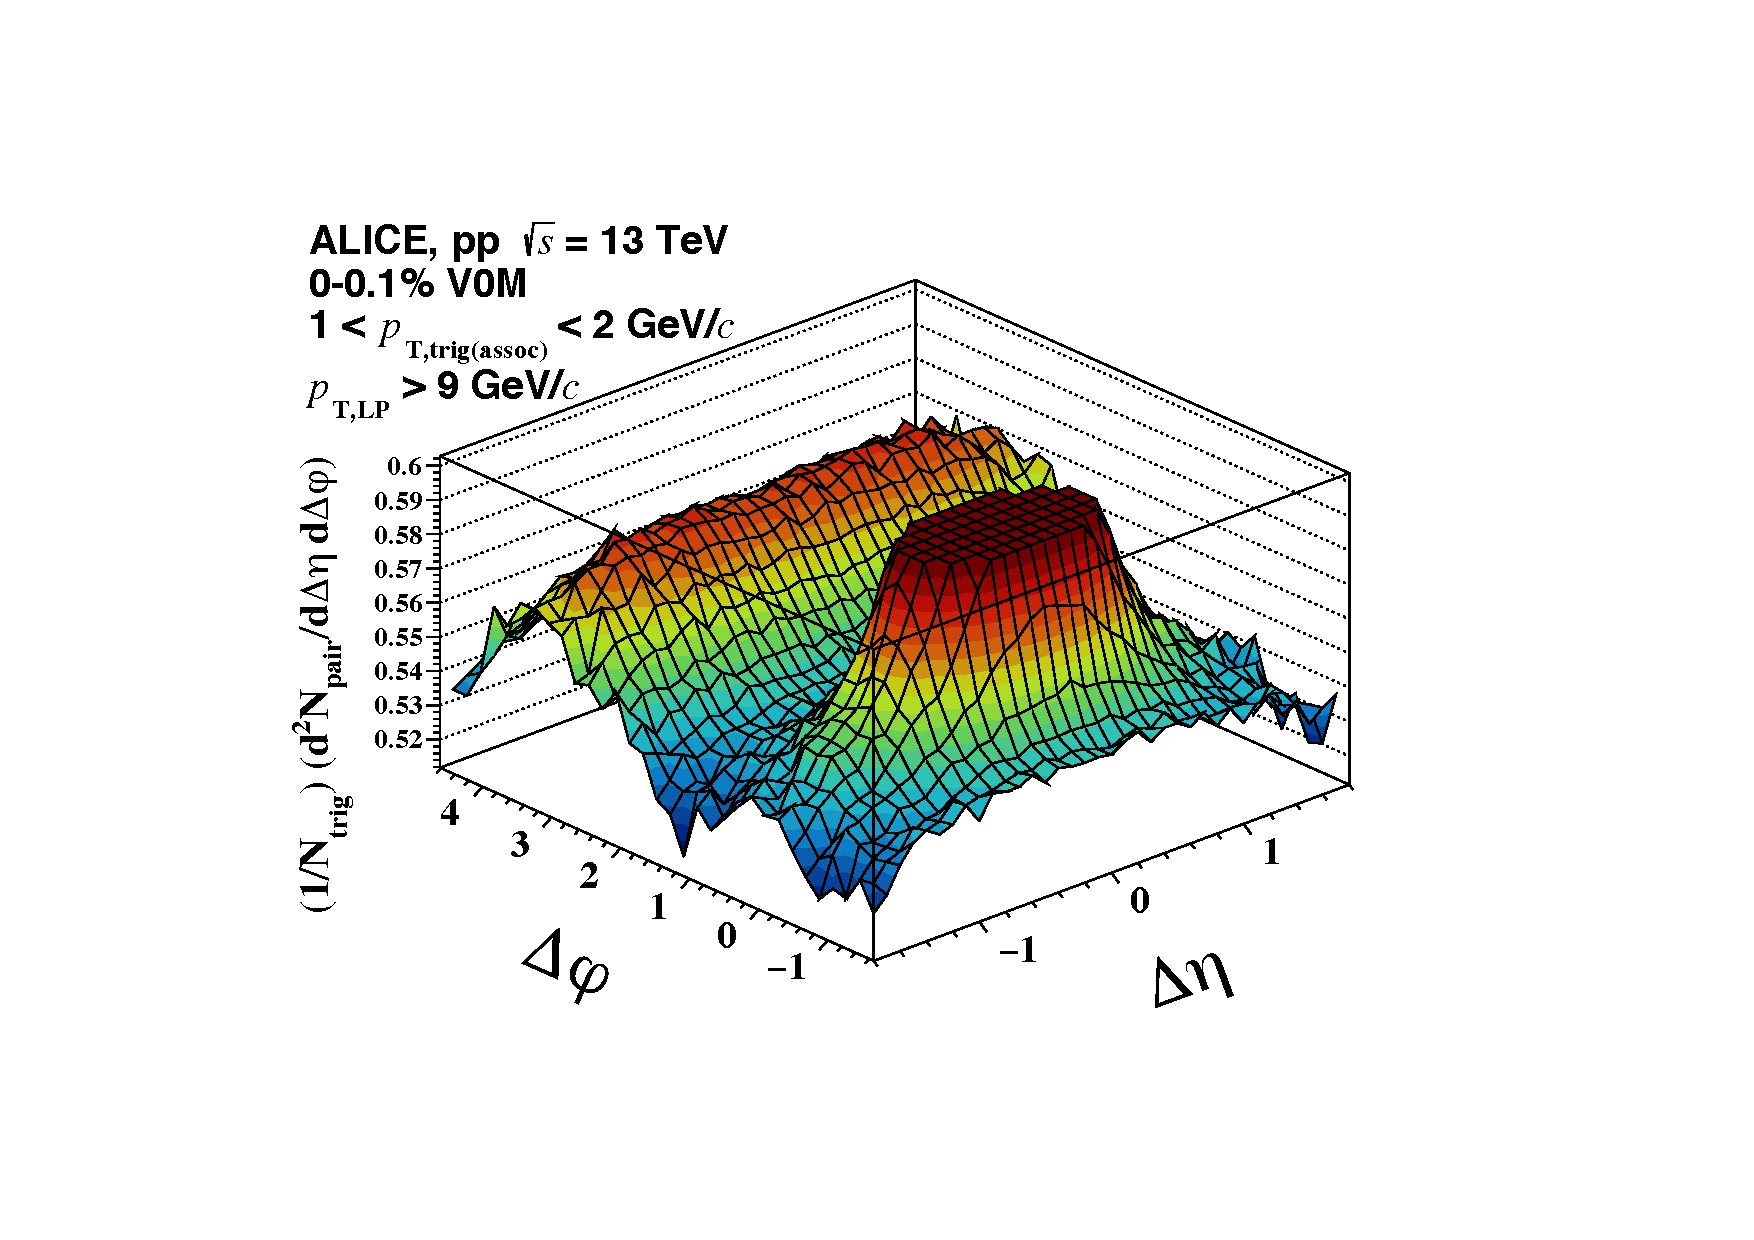
\includegraphics[width=0.47 \textwidth]{./figures/corrlh.pdf} }
	\subfigure{ 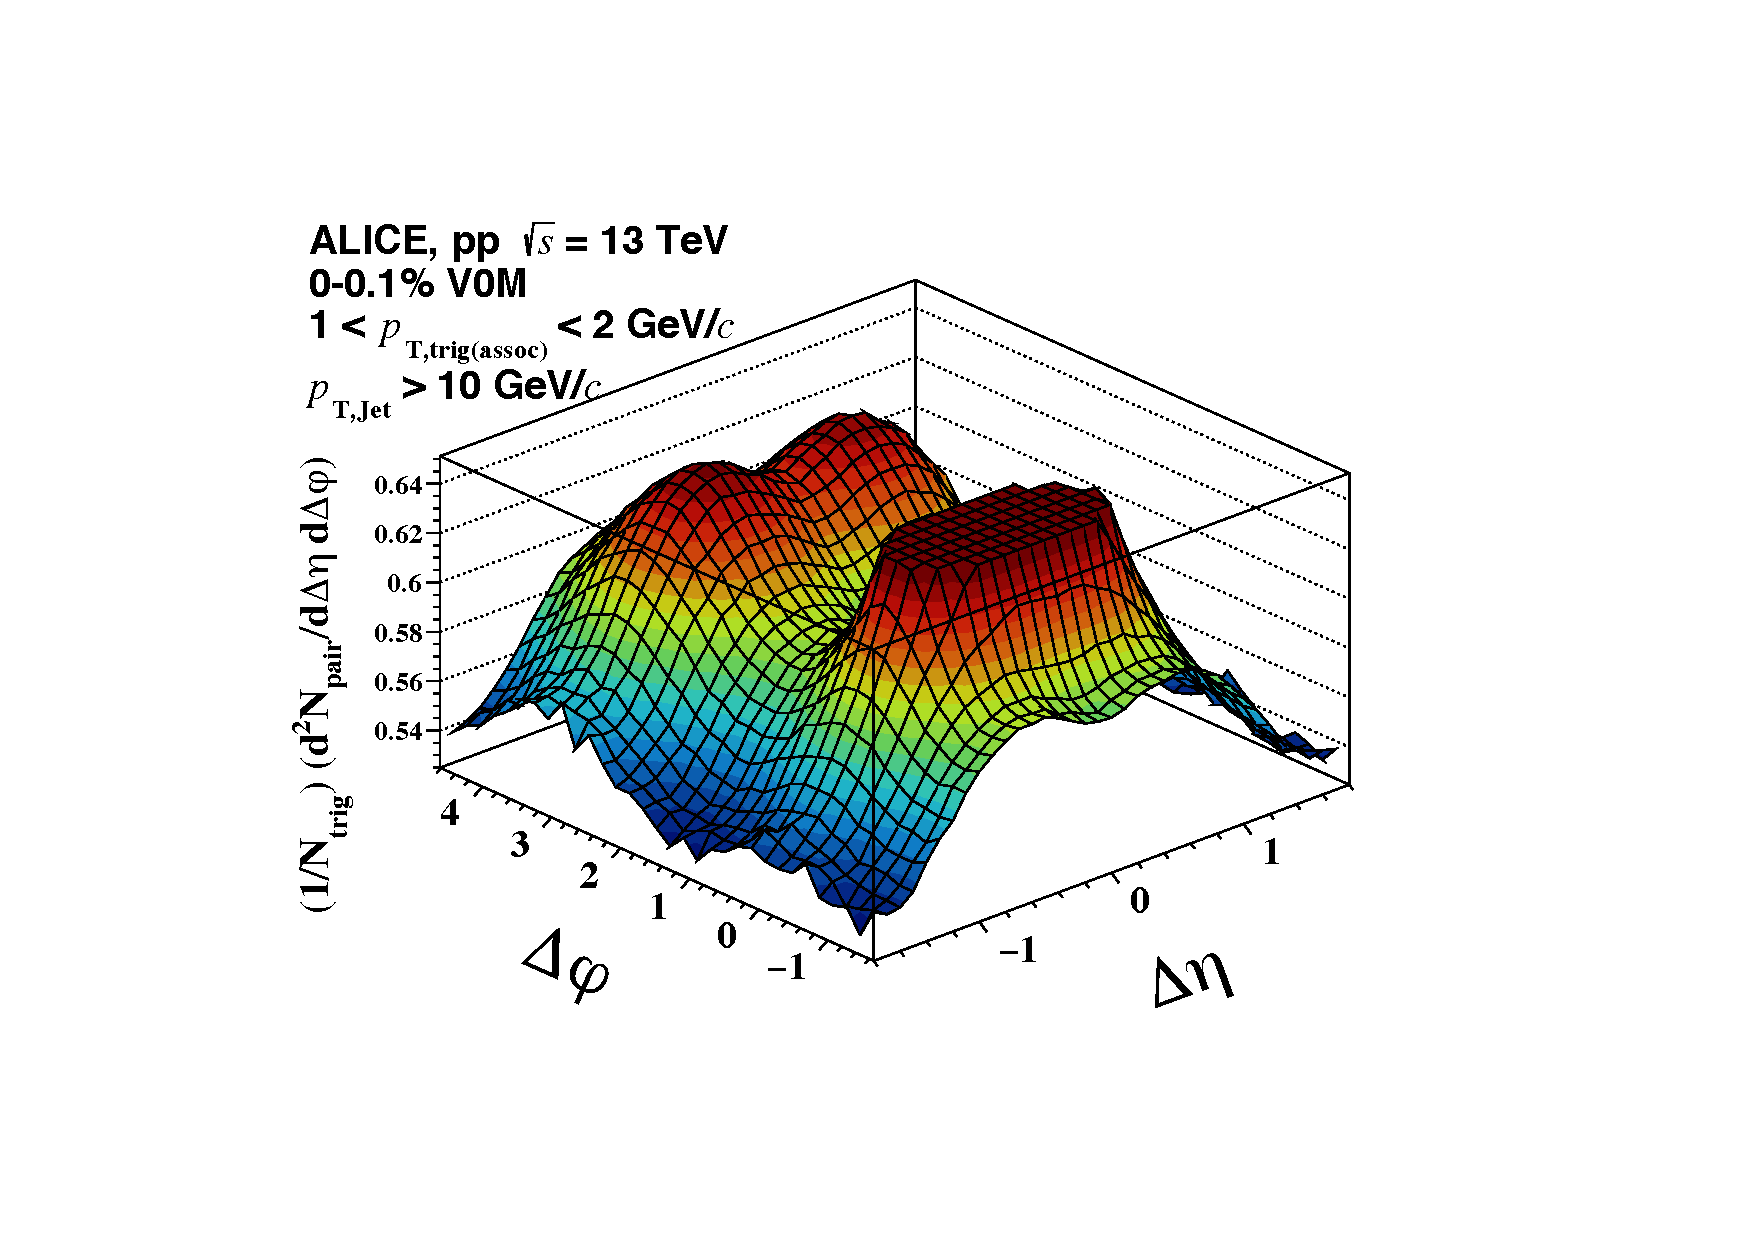
\includegraphics[width=0.47 \textwidth]{./figures/corrjet.pdf} }
	\caption{ Two-dimensional correlation functions as a function of $\Delta\eta$ and $\Delta\varphi$ in high-multiplicity events including a selection on the event-scale. The interval of $\pttrig$ and $\ptassoc$ is 1~$<\pttrigassoc<$~2~GeV/$c$. Left: HM events with a $\ptlead>$~9~GeV/$c$ leading track. Right: HM events with a $\ptjet>$~10~GeV/$c$.}
	\label{fig:PlotCorrHMTSel}
\end{figure}

The ridge yield is further studied with respect to two different event-scales. In the first measurement, the event-scale is set by requiring a minimum $\pt$ cutoff on the leading particle in each event (denoted as $\ptlead$), while in the second measurement, a minimum $\pt$ cutoff is imposed on the leading jet (denoted as $\ptjet$). 

Figure~\ref{fig:PlotCorrHMTSel} shows that the ridge structure for 1~$< \pttrig\,(\ptassoc) <$~2 GeV/$c$ still persists in high-multiplicity pp collisions with $\ptlead>$~9~GeV/$c$ (left) and $\ptjet>$~10~GeV/$c$ (right).  %The interval is the same to the measured ridge yield is maximum without the event-scale selection.
It is worth noting that the correlation function obtained with the minimum $\ptjet$ selection has a double peak structure which is oriented along the $\Delta\eta$ axis at $\Delta\varphi=\pi$. This structure emerges due to the restricted acceptance of the jet tagging, $|\eta_{\rm{jet}}|<$~0.4.

\begin{figure}[h!]
	\centering
	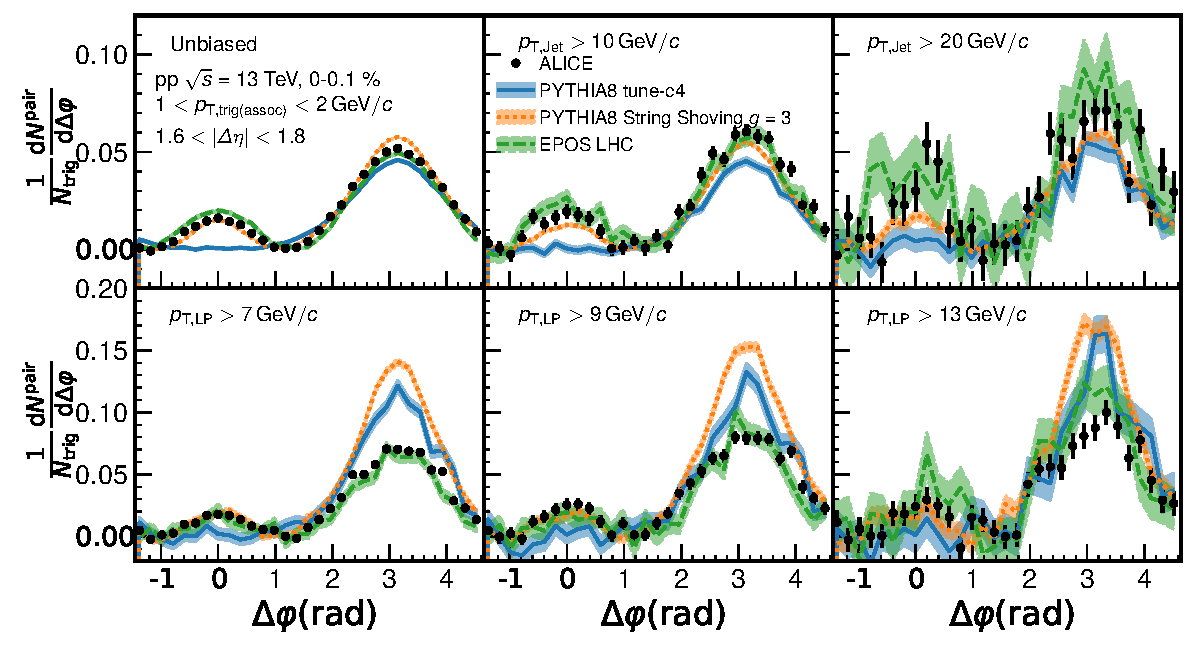
\includegraphics[width=0.99\linewidth]{./figures/Fig5_PlotDeltaPhiESE.pdf}
	\caption{ One-dimensional $\Delta\varphi$ projections of the correlation functions constrained to 1.6~$<|\Delta\eta|<$~1.8 in HM events with an additional event-scale bias. Top: with an imposed selection on the leading jet $\pt$,  bottom: with an imposed selection on the leading particle $\pt$. ALICE data are compared with prediction of models.}
	\label{fig:PlotDeltaPhiESE}
\end{figure}

Figure~\ref{fig:PlotDeltaPhiESE} shows projected $\Delta\varphi$ distributions of the correlation functions in 1.6~$<|\Delta\eta|<$~1.8 with the minimum $\ptlead$ (lower) and $\ptjet$ (upper) requirement. Even with the event-scale selection, the ridge is still visible on the near-side. The near-side ridge peak increases as the thresholds of $\ptlead$ and $\ptjet$ increase compared to the one measured in unbiased events in Sec.~\ref{sec:resultunbiased}. The results are compared with $\pythiashoving$, $\pythiam$, and $\epos$ calculations. The near-side ridge peaks are qualitatively reproduced by $\pythiashoving$ and $\epos$ models. On the other hand, the $\pythiam$ does not show the  near-side ridge peak for neither of the two event-scale selections, but it gives compatible results for the away-side yield just like the $\pythiashoving$ model.

%Both models describe the away-side yield with the $\ptjet$ selection and overestimate away-side yield with the $\ptlead$ selection.

\begin{figure}[h!]
	\centering
	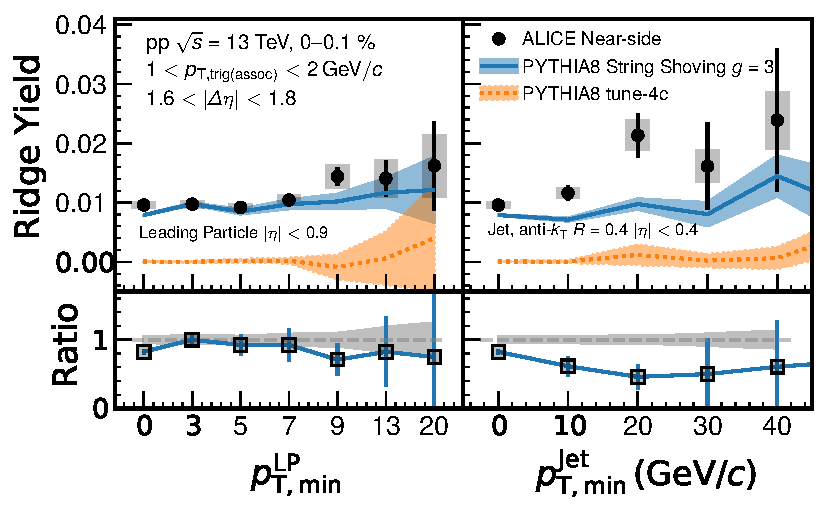
\includegraphics[width=0.89\linewidth]{./figures/Fig6_RidgeYieldESE.pdf}
	\caption{Near-side ridge yield as a function of the $\it{p}^{\rm{LP}}_{\rm{T,min}}$ (left) and $\it{p}^{\rm{Jet}}_{\rm{T,min}}$ (right). Data points (filled circles) show the ALICE measurement. The statistical and systematic uncertainties are shows as vertical bars and boxes, respectively. The upper limit of the jet contamination is not included in the  systematic uncertainty, which is 18.9\%. They are compared with predictions of models which are represented by colored bands. The bottom panel shows a ratio of the models to the data. The uncertainty of the data is represented by the gray band centered around unity.}
	\label{fig:RidgeYield_ESE}
\end{figure}

The ridge yields as function of the minimum $\ptlead$ ($\it{p}^{\rm{LP}}_{\rm{T,min}}$) and $\ptjet$ ($\it{p}^{\rm{jet}}_{\rm{T,min}}$) selections are shown in Fig.~\ref{fig:RidgeYield_ESE}. High-multiplicity events with imposed event-scale bias exhibit increased ridge yields when compared to unbiased HM events. A small increase of the ridge yields as a function of $\ptlead$ or $\ptjet$ is observed and there is no difference between the two event-scale selections within the uncertainties. Comparisons to model calculations show that $\pythiashoving$ provides a comparable trend with data, but underestimates the ridge yield. On the other hand, $\epos$ overestimates the ridge yield while providing a trend comparable with the data. The origin of the enhanced ridge yields for higher momentum jet-tagged events is not clear to date but it might be related to the expected smaller impact parameters for dijet or multi-jet production events as studied in~\cite{Frankfurt:2010ea}.

\begin{figure}[h!]
	\centering
	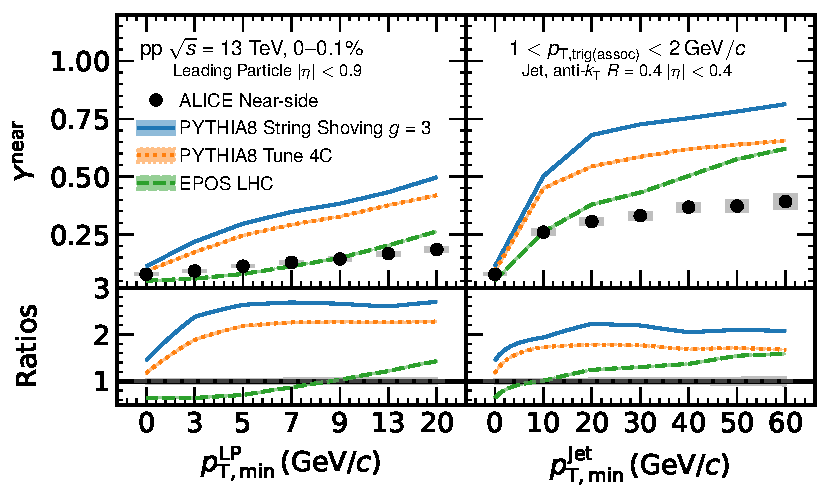
\includegraphics[width=0.89\linewidth]{./figures/Fig9_JetYieldESE.pdf}
	\caption{ Near-side jet-like peak yield as a function of the $\it{p}^{\rm{LP}}_{\rm{T,min}}$ (left) and $\it{p}^{\rm{jet}}_{\rm{T,min}}$ (right). The filled circles show measurement with ALICE. The statistical and systematic uncertainties are shown as vertical bars and boxes, respectively. The measurements are compared with model descriptions from $\pythiam$, $\pythiashoving$, and $\epos$ for both selections. The total uncertainty of the ratio is represented by the gray band centered around unity.}
	\label{fig:JetYield_ESE}
\end{figure}

Finally, the near-side jet-like peak yield is measured as a function of minimum $\ptlead$ and $\ptjet$ in Fig.~\ref{fig:JetYield_ESE} to further test the models that aim to describe the near-side ridge. $\epos$ provides comparable estimates of the near-side jet-like peak yield, while $\pythiam$ and $\pythiashoving$ overestimate the near-side yields for both event selections.

In all models if the ridge is due to final-state interactions, e.g., $\epos$ and PYTHIA~8 String Shoving, one also expects the near-side jet-like peak yield to be affected. This can be observed when comparing the measured near-side jet yields with PYTHIA~8 calculations with and without String Shoving. The new ALICE results therefore provide constraints beyond traditional ridge measurements that challenge existing models.